%!TEX root = ../thesis.tex
\chapter{Applications \& Discussion}

This chapter presents a discussion of the GUIs software design and its consequences for musical mapping. The interface's features are explored in an attempt to evaluate the successes and failures of the design. Each subview 

%%%%%%%%%%%%%%%%%%%%%%%%%%%%%%%%%%%%%%%%%%%%%%%%%%%%%%%%%%%%%%%%%%%%%%%%%%%%%%%%%%%%%%%%%%%%%%%%%%%%%%%%%%%%%%%%%%%%%%%%%%%%%%%%%%%%%%%%%%%%%%%%%%%%%%%%%%%%%%%%%%%%%%%%%%%%%%%%%%%%%%%%%%%%%%%%%%%%%%%%%%%%%%%%%%%%%%%%%%%%%%%%%%%%%%%%%%%%%%%%%%%%%%%%%%%%%%%%%%
\section{Effectiveness of Alternate Views} % (fold)
\label{sec:effectiveness_of_alternate_views}

	\subsection{List view} % (fold)
	\label{sub:list_view}

%list view weaknesses
%	intermediate devices
%	heirarchical structures
%	many-to-one mappings
	
	% subsection list_view (end)

	\subsection{Grid view} % (fold)
	\label{sub:grid_view}
	
	% subsection grid_view (end)

	\subsection{Hive view} % (fold)
	\label{sub:hive_view}

	% bogs down the network with requests
	
	% subsection hive_view (end)

% section effectiveness_of_alternate_views (end)

%%%%%%%%%%%%%%%%%%%%%%%%%%%%%%%%%%%%%%%%%%%%%%%%%%%%%%%%%%%%%%%%%%%%%%%%%%%%%%%%%%%%%%%%%%%%%%%%%%%%%%%%%%%%%%%%%%%%%%%%%%%%%%%%%%%%%%%%%%%%%%%%%%%%%%%%%%%%%%%%%%%%%%%%%%%%%%%%%%%%%%%%%%%%%%%%%%%%%%%%%%%%%%%%%%%%%%%%%%%%%%%%%%%%%%%%%%%%%%%%%%%%%%%%%%%%%%%%%%
\section{User Feedback} % (fold)
\label{sec:user_feedback}

%began and informed our entire process, feedback from prior guis and projects has been alluded to and is important presented here is feedback for our GUI

	\subsection{Present use cases} % (fold)
	\label{sub:present_use_cases}

		%Mailis, Clayton, Hakon, Julie

	% subsection present_user_applications (end)

	\subsection{Saving \& loading} % (fold)
	\label{sub:saving_and_loading}
	
	% subsection saving_&_loading (end)

	\subsection{Reliability \& Responsiveness} % (fold)
	\label{sub:reliability_and_responsiveness}
	
	% subsection reliability_and_responsiveness (end)

	\subsection{Other feedback} % (fold)
	\label{sub:other_feedback}
	
	% subsection other_feedback (end)
	
% section user_feedback (end)

%%%%%%%%%%%%%%%%%%%%%%%%%%%%%%%%%%%%%%%%%%%%%%%%%%%%%%%%%%%%%%%%%%%%%%%%%%%%%%%%%%%%%%%%%%%%%%%%%%%%%%%%%%%%%%%%%%%%%%%%%%%%%%%%%%%%%%%%%%%%%%%%%%%%%%%%%%%%%%%%%%%%%%%%%%%%%%%%%%%%%%%%%%%%%%%%%%%%%%%%%%%%%%%%%%%%%%%%%%%%%%%%%%%%%%%%%%%%%%%%%%%%%%%%%%%%%%%%%%
\section{Testing program responsiveness} % (fold)
\label{sec:testing_program_responsiveness}

Extension of interface features discussed in section \ref{sec:extension_of_control_and_visual_elements} leads to some control possibilities that could be difficult for the GUI to handle. Addition of shortcut keys for connecting, linking, disconnecting and unlinking, as well as the ability to select multiple devices and signals at once allows users to create and delete hundreds of connections with a single keypress. Na\"{i}ve saving and loading produces to situations where dense mappings will accidentally be applied to several instruments at once.

Though the ``update display'' model works extremely well for code modularity, it generates awkward situations when dealing with massive network operations. Since the system updates the entire display with each change to the network, deleting 100 links (if the user is clearing a large network) results in 100 independent \url{delete_link} messages arriving at the monitor. For each one of these messages, the display will fully update. In the case of the list view mode, all arrows will be cleared, and redrawn with one fewer present (as if the links are being deleted one-by-one). In total 4950 arrow drawing operations\footnote{$99 + 98 + 97 + ... + 2 + 1 = \frac{99*100}{2}$. Note that $\frac{n*(n+1)}{2}$ arrows will be drawn for any $n$ number of arrows.} will occur, resulting in siginificant delay. 

As reported by users in section \ref{sub:reliability_and_responsiveness}, any GUI operation that takes more than a few seconds, without some kind of visual feedback (like a ``loading'' bar), leads to frustration and mistrust of the program. Obviously, if the GUI is going to support these kinds of massive network manipulations, there needs to exist some way to keep them under control.

	\subsection{Rate limiting certain functions} % (fold)
	\label{sub:rate_limiting_certain_functions}

In order to prevent thousands of uneccesary, display re-draws, a ``waiting'' period was added to certain critical functions. This operating systems process is described in \shortciteN{os_concepts}. Essentially certain functions no longer execute in the code immediately once called, instead, a delay timer starts. If the function is called again during this delay, the delay timer simply restarts. The function is only executed once the delay timer finishes. This way, if a function is called 100 times simultaneously, it will only execute once after a short delay. Figure \ref{fig:waiting_period} shows the effect of the waiting period if the function is called a single time, and if it is called once during the delay.

\begin{figure}[ht]
	\centering
		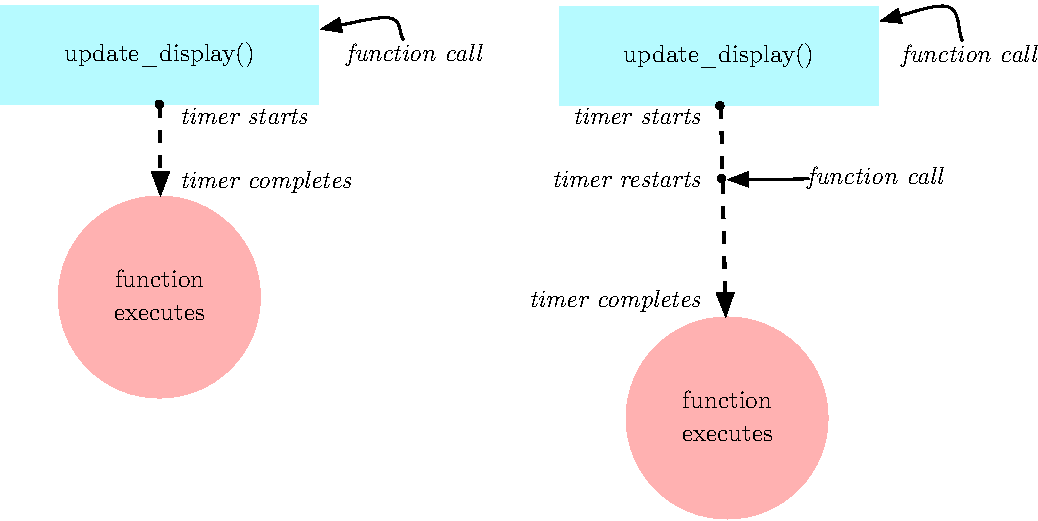
\includegraphics[width=1\textwidth]{figures/waiting_period}
		\caption{Illustration of a delayed function.}
		\label{fig:waiting_period}
\end{figure}

Two functions are limited in the GUI: \url{update_display} for all views and \url{update_arrows} for the list view. \url{update_display} is common to all views, and the massive network changes described above can result in many processor intesive functions to run needlessly. With the \url{update_arrows} function, operations that do not result in changes to the network (scrolling, changing tabs) require constant re-drawing.

Exactly how much time this delay should be set to is not obvious. If the delay is too short it is possible for massive network operations to still call the function many times if they arrive asynchronously. A too-long delay means that users may notice for simple actions, like scrolling with a single arrow (causing the srolling to appear jerky). Another consequence of a long delay is that a process which calls the delayed function at a reglar interval could continuously restart the delay. In this case the function will \emph{never} execute, a situation known as ``starvation'' \shortcite{os_concepts}.
	
	% subsection rate_limiting_certain_functions (end)

	\subsection{A test case: creation of many arrows in the list view} % (fold)
	\label{sub:test_case}

To best determine the length of the function waiting periods, a simple test was conducted. Several

	% subsection test_case (end)

% section testing_program_responsiveness (end)

%%%%%%%%%%%%%%%%%%%%%%%%%%%%%%%%%%%%%%%%%%%%%%%%%%%%%%%%%%%%%%%%%%%%%%%%%%%%%%%%%%%%%%%%%%%%%%%%%%%%%%%%%%%%%%%%%%%%%%%%%%%%%%%%%%%%%%%%%%%%%%%%%%%%%%%%%%%%%%%%%%%%%%%%%%%%%%%%%%%%%%%%%%%%%%%%%%%%%%%%%%%%%%%%%%%%%%%%%%%%%%%%%%%%%%%%%%%%%%%%%%%%%%%%%%%%%%%%%%
\section{Comparison to Similar Interfaces} % (fold)
\label{sec:comparison_to_similar_interfaces}

	\subsection{Junxion} % (fold)
	\label{sub:junxion}
		\cite{junxion}
	% subsection junxion (end)

	\subsection{Osculator} % (fold)
	\label{sub:osculator}
		\cite{osculator}
	% subsection osculator (end)

	\subsection{Other similar interfaces} % (fold)
	\label{sub:other_similar_interfaces}
	
	\begin{enumerate}
		\item Inclusive interconnections \shortcite{inclusiveinterconnections}
		\item Sense Stage \shortcite{senseStage}
		\item mpgcarepackage?
		\item Integra \shortcite{integra}
		\item Eaganmatrix: GRID VIEW! \shortcite{eaganmatrix}
		\item Patchage: a linking, dragging, connecting interface \shortcite{patchage}
	\end{enumerate}

	% subsection other_similar_interfaces (end)

% section comparison_to_similar_interfaces (end)

%%%%%%%%%%%%%%%%%%%%%%%%%%%%%%%%%%%%%%%%%%%%%%%%%%%%%%%%%%%%%%%%%%%%%%%%%%%%%%%%%%%%%%%%%%%%%%%%%%%%%%%%%%%%%%%%%%%%%%%%%%%%%%%%%%%%%%%%%%%%%%%%%%%%%%%%%%%%%%%%%%%%%%%%%%%%%%%%%%%%%%%%%%%%%%%%%%%%%%%%%%%%%%%%%%%%%%%%%%%%%%%%%%%%%%%%%%%%%%%%%%%%%%%%%%%%%%%%%%
\section{Evaluation of Goals} % (fold)
\label{sec:evaluation_of_goals}
	Are sections graphically unified? (Is this even necessary?)
	%Why is what what on the top bar`'

% section evaluation_of_goals (end)




